\documentclass{beamer}

\usetheme{default}

\usefonttheme{structurebold}
\usepackage{helvet}
\usecolortheme{seagull}         % white on black

\usepackage[utf8]{inputenc}
\PassOptionsToPackage{hyphens}{url}\usepackage{hyperref,xspace,multicol}
\usepackage[absolute,overlay]{textpos}
\usepackage{tikz}
\usetikzlibrary{arrows,shapes,trees,shadows,positioning}
%% \usepackage{tree}
\usepackage{fancyvrb}           % for \Verb

% Remember the position of every picture.
\tikzstyle{every picture}+=[remember picture]

\tikzset{onslide/.code args={<#1>#2}{%
  \only<#1>{\pgfkeysalso{#2}} % \pgfkeysalso doesn't change the path
}}

% Colors.
\definecolor{guixred1}{RGB}{226,0,38}  % red P
\definecolor{guixorange1}{RGB}{243,154,38}  % guixorange P
\definecolor{guixyellow}{RGB}{254,205,27}  % guixyellow P
\definecolor{guixred2}{RGB}{230,68,57}  % red S
\definecolor{guixorange2}{RGB}{236,117,40}  % guixorange S
\definecolor{guixtaupe}{RGB}{134,113,127} % guixtaupe S
\definecolor{guixgrey}{RGB}{91,94,111} % guixgrey S
\definecolor{guixblue1}{RGB}{38,109,131} % guixblue S
\definecolor{guixblue2}{RGB}{10,50,80} % guixblue S
\definecolor{guixgreen1}{RGB}{133,146,66} % guixgreen S
\definecolor{guixgreen2}{RGB}{157,193,7} % guixgreen S

\setbeamerfont{title}{size=\huge}
\setbeamerfont{frametitle}{size=\huge}

% Black-on-white color theme.
\setbeamercolor{structure}{fg=guixblue2}
\setbeamercolor{title}{fg=guixblue2}
\setbeamercolor{frametitle}{fg=guixblue2}
\setbeamercolor{date}{fg=darkgray}
\setbeamercolor{author}{fg=darkgray}
\setbeamercolor{alerted text}{fg=guixblue2,bg=black}

% White-on-black color theme.
%% \setbeamercolor{structure}{fg=guixorange1,bg=black}
%% \setbeamercolor{title}{fg=white,bg=black}
%% \setbeamercolor{date}{fg=guixorange1,bg=black}
%% \setbeamercolor{frametitle}{fg=white,bg=black}
%% \setbeamercolor{titlelike}{fg=white,bg=black}
%% \setbeamercolor{normal text}{fg=white,bg=black}
%% \setbeamercolor{alerted text}{fg=guixyellow,bg=black}
%% \setbeamercolor{section in toc}{fg=white,bg=black}
%% \setbeamercolor{section in toc shaded}{fg=white,bg=black}
%% \setbeamercolor{subsection in toc}{fg=guixorange1,bg=black}
%% \setbeamercolor{subsection in toc shaded}{fg=white,bg=black}
%% \setbeamercolor{subsubsection in toc}{fg=guixorange1,bg=black}
%% \setbeamercolor{subsubsection in toc shaded}{fg=white,bg=black}
%% \setbeamercolor{frametitle in toc}{fg=white,bg=black}
%% \setbeamercolor{local structure}{fg=guixorange1,bg=black}


\title{The Emacs of Distros}
\subtitle{How GNU Guix Seeks to Empower Users}

\author{Ludovic Courtès\\\texttt{ludo@gnu.org}}
\date{\small{FOSDEM\\31 January 2015}}

\setbeamertemplate{navigation symbols}{} % remove the navigation bar

\AtBeginSection[]{
  \begin{frame}
    \frametitle{}
    \tableofcontents[currentsection, hideothersections]
  \end{frame} 
}


\AtBeginSubsection[]{
  \begin{frame}
  \frametitle{}
  \tableofcontents[currentsection, currentsubsection]
  \end{frame}
}

\begin{document}

\maketitle

\begin{frame}[fragile]

  \huge{\textbf{Emacs Makes\\All Computing Simple!}}
  \\[1.3cm]
  \uncover<2>{\large{or Emacs Makes A Computer Slow?}}
\end{frame}

\begin{frame}[fragile]
  \uncover<2->{\huge{\textbf{freedom \#1} $\rightarrow$ \textbf{system design}}}
  \\[1cm]
  \begin{enumerate}
    \setcounter{enumi}{-1}
  \item run
  \item \textbf<2->{study \& modify}
  \item redistribute
  \item redistribute modified versions
  \end{enumerate}
\end{frame}

\begin{frame}[fragile]
  \textrm{\LARGE{\textbf{ When large numbers of nontechnical workers are
        using a programmable editor, they will be tempted constantly
        \alert{to begin programming} in the course of their day-to-day
        lives.  This should contribute greatly to computer literacy
        [...]
      %% [Many] of the people thus exposed [to Emacs] will be secretaries
      %% taught by society that they are incapable of doing mathematics,
      %% and unable to imagine for a moment that they can learn to program.
      %% \textbf{But that won't stop them from learning} it if they don't
      %% know that it is programming that they are learning!
  }}}

  \vspace{1cm}
  \hfill{-- Stallman, 1981}
\end{frame}

\begin{frame}[plain]
  \center{
\includegraphics[height=0.8\textheight]{images/gnuhead}}
\end{frame}

\begin{frame}{the barriers to distro hacking}
  \Large{
  \begin{itemize}
  \item \textbf{packaging}, ability to \textbf{extend}
  \item \textbf{package management tools}
  \item \textbf{esoteric configuration}
  \item \textbf{implementation language barriers}
  \end{itemize}
  }
\end{frame}

\begin{frame}[plain]
  
\includegraphics[width=\textwidth]{images/guix-logo}
\end{frame}

\setbeamercolor{normal text}{fg=white,bg=guixyellow}
\begin{frame}[plain]
  \Huge\alert{\texttt{M-x guix-demo}}
\end{frame}
\setbeamercolor{normal text}{fg=black,bg=white}

\begin{frame}[fragile, t]
  \frametitle{workflow}

  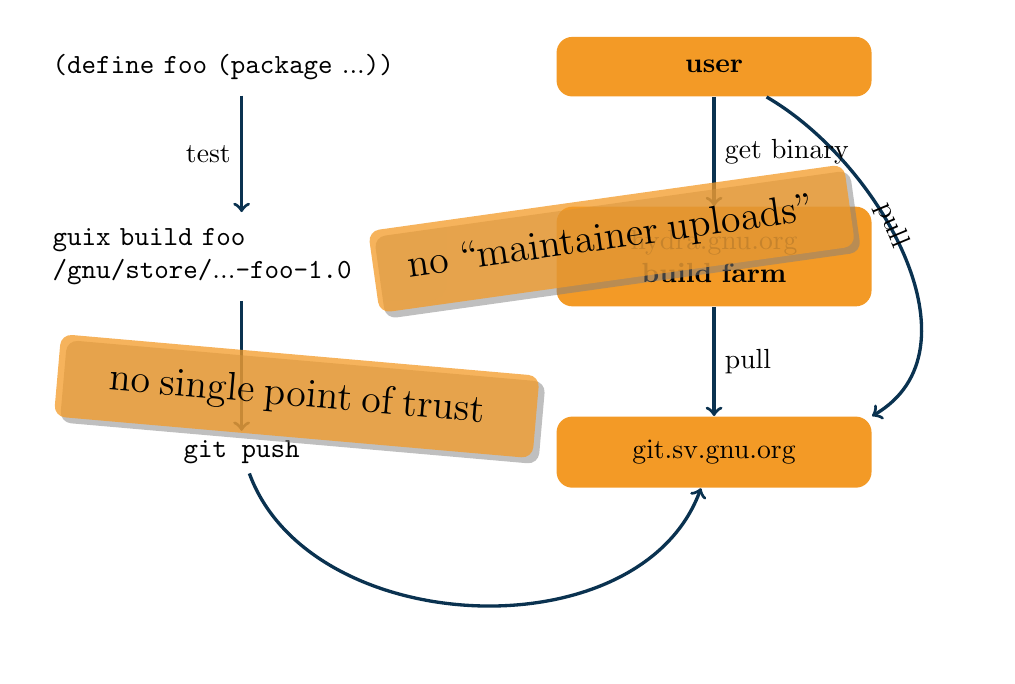
\begin{tikzpicture}[box/.style = {
                         rounded corners=2mm,
                         fill=white, text=black, text width=4.8cm,
                         inner sep=2mm
                      },
                      server/.style = {
                         text centered, rounded corners=2mm,
                         fill=guixorange1, text=black, text width=3.4cm,
                         inner sep=3mm
                      },
                      note/.style = {
                        rounded corners=4, text centered,
                        fill=guixorange1, text width=5.5cm,
                        inner sep=3mm, rotate=5, opacity=.75, text opacity=1,
                        drop shadow={opacity=0.5}
                      }]
    \matrix[row sep=1.4cm, column sep=1.4cm] {
      \node(def)[box]{\texttt{(define foo (package \textrm{...}))}};
      & \node(user)[server]{\textbf{user}};
      \\
      \node<2->(build)[box]{\texttt{guix build foo}
         \texttt{/gnu/store/\textrm{...}-foo-1.0}};
      & \node<4-5>(hydra)[server]{hydra.gnu.org \textbf{build~farm}};
      \\
      \node<3->(push){\texttt{git push}};
      & \node<3->(savannah)[server]{git.sv.gnu.org}; \\
      \\
    };

    \path[->, very thick, draw=guixblue2]<2->
      (def) edge node[left]{test} (build);
    \path[->, very thick, draw=guixblue2]<3->
      (build) edge (push);
    \path[->, very thick, draw=guixblue2]<3->
      (push) edge[->, in=-110, out=-70] (savannah);
    \path[->, very thick, draw=guixblue2]<4-5>
      (hydra) edge node[right]{pull} (savannah);
    \path[->, very thick, draw=guixblue2]<4-6>
      (user) edge[in=30,out=-30] node[left, sloped]{pull}
      (savannah.north east);
    \path[->, very thick, draw=guixblue2]<5>
      (user) edge node[right]{get binary} (hydra);

    \node<7>[note, rotate=3] at (2,1) {\Large{no ``maintainer uploads''}};
    \node<7>[note, rotate=-10] at (-2,-1) {\Large{no single point of trust}};
  \end{tikzpicture}
\end{frame}

\begin{frame}[fragile]
  \frametitle{reproducible builds$^*$}
  \framesubtitle{$^*$ almost!}

  \begin{semiverbatim}
\$ guix build guile
\uncover<2->{/gnu/store/\tikz[baseline]{\node[anchor=base](nixhash){\alert<2>{h2g4sc09h4...}};}-guile-2.0.11}

\uncover<3->{\$ \alert<3>{guix gc --references /gnu/store/...-guile-2.0.11}
/gnu/store/4jl83jgzaac...-glibc-2.20
/gnu/store/iplay43cg58...-libunistring-0.9.3
/gnu/store/47p47v92cj9...-libffi-3.0.9
/gnu/store/drkwck2j965...-gmp-5.0.5
...}
  \end{semiverbatim}

  \begin{tikzpicture}[overlay]
    \node<1>(labelnixhash) [fill=white, text=black] at (current page.center) {%
      \Large{\textbf{isolated build}: chroot, separate name spaces, etc.}
    };

    \node<2>(labelnixhash) [fill=white, text=black] at (4cm, 2cm) {%
      hash of \textbf{all} the dependencies};
    \path[->]<2>(labelnixhash.north) edge [bend left, in=180, out=-45] (nixhash.south);

    \draw<4> (-10pt, 105pt) [very thick, color=guixorange2, rounded corners=8pt]
      arc (10:-50:-50pt and 110pt);
    \node<4>[fill=black, text=white, text opacity=1, opacity=.7,
          rounded corners=2mm, inner sep=5mm]
      at (7, 2) {\textbf{\Large{(nearly) bit-identical for everyone}}};
  \end{tikzpicture}

\end{frame}


\begin{frame}[plain]
  \begin{tikzpicture}[overlay]
    % http://www.heise.de/ct/artikel/NSA-GCHQ-The-HACIENDA-Program-for-Internet-Colonization-2292681.html?hg=1&hgi=8&hgf=false
    \node [at=(current page.center), inner sep=0mm]
    {\includegraphics[height=\paperheight]{images/sigint-rice}};

    %% \node<2>[rounded corners=4, text centered,
    %%       fill=guixorange1, text width=10cm,
    %%       inner sep=2mm, rotate=5, opacity=.75, text opacity=1,
    %%       drop shadow={opacity=0.5}] at (current page.center) {
    %%   \LARGE{\textbf{do not \alert{trust} a single\\ binary provider}}
    %% };
  \end{tikzpicture}
\end{frame}

\setbeamercolor{normal text}{fg=white,bg=guixyellow}
\begin{frame}[plain]
  \Huge{\alert{\texttt{M-x hack-the-distro}}}
\end{frame}
\setbeamercolor{normal text}{fg=black,bg=white}

\begin{frame}[fragile]{}
  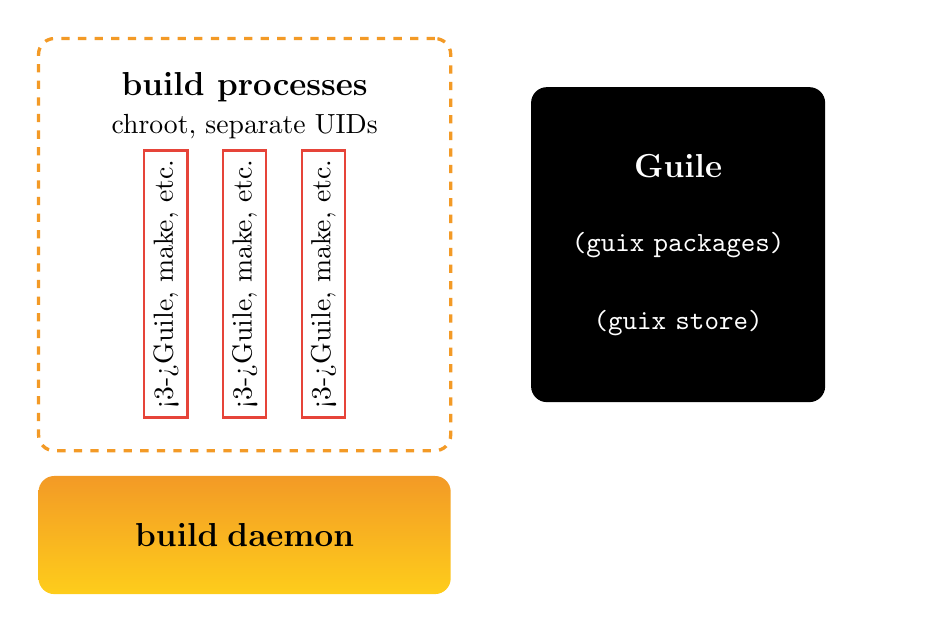
\begin{tikzpicture}[tools/.style = {
                        text width=35mm, minimum height=4cm,
                        text centered,
                        rounded corners=2mm,
                        fill=black, text=white
                      },
                      tool/.style = {
                        fill=black, text=white, text width=3cm,
                        text centered
                      },
                      daemon/.style = {
                        rectangle, text width=50mm, text centered,
                        rounded corners=2mm, minimum height=15mm,
                        top color=guixorange1,
                        bottom color=guixyellow,
                        text=black
                      },
                      builders/.style = {
                        draw=guixorange1, very thick, dashed,
                        fill=white, text=black, text width=5cm,
                        rounded corners=2mm,
                      },
                      builder/.style = {
                        draw=guixred2, thick, rectangle,
                        fill=white, text=black,
                        rotate=90
                      }]
    \matrix[row sep=3mm, column sep=1cm] {
      \node(builders)[builders, text height=5cm]{}
          node at (0, 2) {\large{\textbf{build processes}}}
          node at (0, 1.5) {chroot, separate UIDs}
          node[builder, onslide=<1-2>{white}] at (-1,-0.5) {\alert<3->{Guile}, make, etc.}
          node[builder, onslide=<1-2>{white}] at ( 0,-0.5) {\alert<3->{Guile}, make, etc.}
          node[builder, onslide=<1-2>{white}] at ( 1,-0.5) {\alert<3->{Guile}, make, etc.}; &
      \node[tools]{}
          node[text=white] at (0, 1) {\large{\textbf{Guile}}}
          node[tool] at (0, 0) {\texttt{(guix packages)}}
          node(client)[tool] at (0, -1) {\texttt{(guix store)}};
      \\

      \node(daemon)[daemon]{\large{\textbf{build daemon}}}; &
      &
      \\
    };
  \end{tikzpicture}

  \begin{tikzpicture}[overlay]
    \path[very thick, draw=guixblue2]<2->
      (client.south) edge [out=-90, in=0, ->] node[below, sloped]{RPCs} (daemon.east);
    \path[->, very thick, draw=guixblue2]<3->
      (daemon) edge (builders);
  \end{tikzpicture}
\end{frame}

\setbeamercolor{normal text}{fg=white,bg=guixyellow}
\begin{frame}[plain]
  \hspace{-0.5cm}
  \Huge{\alert{\texttt{M-x customize-operating-system}}}
\end{frame}
\setbeamercolor{normal text}{fg=black,bg=white}

\begin{frame}[fragile]
  \begin{overlayarea}{\textwidth}{8cm}
  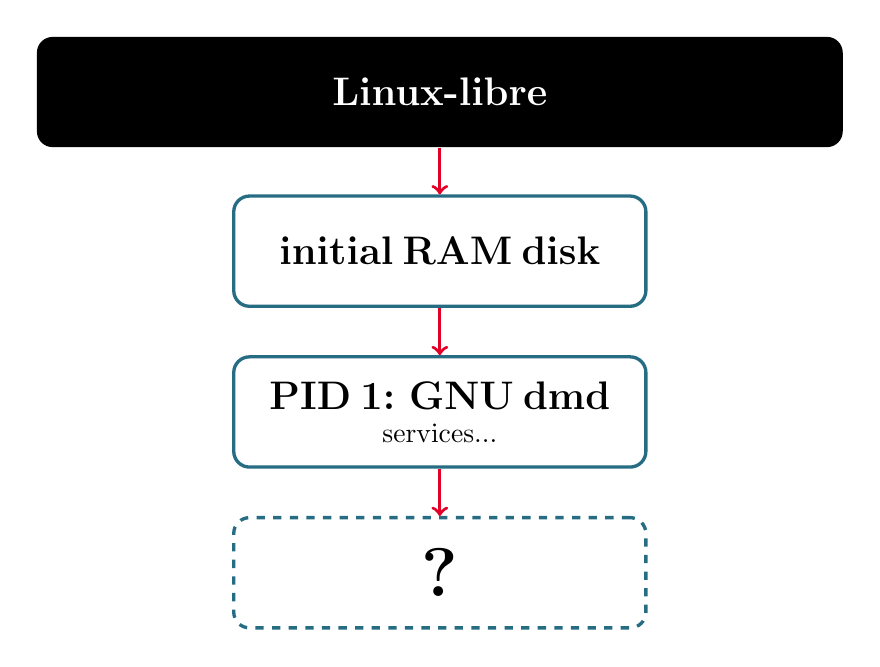
\begin{tikzpicture}[kernel/.style = {
                        text width=10cm, minimum height=1.4cm,
                        text centered,
                        rounded corners=2mm,
                        fill=black, text=white
                      },
                      userland/.style = {
                        draw=guixblue1, very thick,
                        fill=white, text=black, text width=5cm,
                        rounded corners=2mm, minimum height=1.4cm,
                        text centered
                      }]
    \matrix[row sep=6mm, column sep=1cm] {
      \node(kernel)[kernel]{\textbf{\Large{Linux-libre}}};
      \\

      \node<2->(initrd)[userland]{\textbf{\Large{initial RAM disk}}};
      \\

      \node<4->(dmd)[userland]{\textbf{\Large{PID 1: GNU dmd}}
        \\ services...};
      \\

      \node<6->(user)[userland, dashed]{\Huge{\textbf{?}}};
      \\
    };

    \path[->, very thick, draw=guixred1]<2->
      (kernel) edge (initrd);
    \path[->, very thick, draw=guixred1]<4->
      (initrd) edge (dmd);
    \path[->, very thick, draw=guixred1]<6->
      (dmd) edge (user);
    
  \end{tikzpicture}
  \end{overlayarea}

  \begin{tikzpicture}[overlay,
                      guile/.style = {
                         fill=guixyellow, text=black, rotate=30,
                         rounded corners=4mm, text width=3cm,
                         opacity=.75, text opacity=1, text centered,
                         minimum height=1.3cm
                      }]
    \node<3->(labelinitrd) [guile] at (initrd.east) {%
      \Large{Guile!}
    };
    \node<5->(labelinitrd) [guile] at (dmd.east) {%
      \Large{Guile!}
    };
  \end{tikzpicture}
\end{frame}

%%%%%%%%%%%%%%%%%%%%%%%%%%%%%%%%%%%%%%%%%%%%%%%%%%%%%%%%%%%%%%%%%%%%%%%%%%%%%%%%
\setbeamercolor{normal text}{fg=white,bg=guixyellow}
\begin{frame}[plain]
  \hspace{-0.5cm}
  \Huge{\alert{\texttt{M-x guix-status}}}
\end{frame}
\setbeamercolor{normal text}{fg=black,bg=white}

\begin{frame}{timeline}
  \begin{itemize}
    \item Nov. 2012 --- dubbed GNU
    \item{Jan. 2013 --- \alert{0.1}}
    \item ...
    \item{Apr. 2014 --- \alert{0.6}, signed binaries, \texttt{guix
        system}}
    \item{July 2014 --- \alert{0.7}, \textbf{installable operating
        system!}}
    \item{Nov. 2014 --- \alert{0.8}, device mapping, more services,
      etc.}
    \item<2->{29 Jan. 2015 --- \alert{0.8.1}, \textbf{ARMv7 port, bug
        fixes}}
    \item<3->{30 Jan. 2015 --- officially \textbf{FSDG-compliant}!}
  \end{itemize}
\end{frame}


\begin{frame}[plain]
  \frametitle{status}
  \begin{tikzpicture}[overlay]
    % http://en.wikipedia.org/wiki/File:Kibbles_How_Others_See_Me.jpg
    \node [at=(current page.center), inner sep=0mm]
    {\includegraphics[width=\paperwidth]{images/dog-food}};

    \node [text=white] at (current page.center) { \Huge{\textbf{status}} };
  \end{tikzpicture}
\end{frame}

\begin{frame}{status}
  \Large{
  \begin{itemize}
    \item full-featured package manager
    \item 1,200 packages, 4 platforms
    \item \textbf{Guix System Distribution$^\beta$}
    \item binaries at \url{http://hydra.gnu.org}
    \item tooling: auto-update, ``linting'', etc.
    \item l10n: 8 languages!
  \end{itemize}}
\end{frame}

\begin{frame}[plain]
  \begin{tikzpicture}[overlay]
    % https://www.openhub.net/p/gnuguix
    \node [at=(current page.center), inner sep=0mm]
    {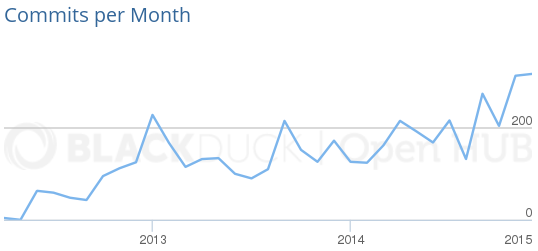
\includegraphics[width=0.9\paperwidth]{images/openhub-commits}};
  \end{tikzpicture}
\end{frame}

\begin{frame}[plain]

  \begin{tikzpicture}[remember picture, overlay]
    \node [at=(current page.center), inner sep=0pt]
      {
\includegraphics[width=\paperwidth]{images/openhub-activity}};
  \end{tikzpicture}
\end{frame}

\begin{frame}{thanks for the code, reports, ideas, build machines...}

  \begin{itemize}
    \item Eric Bavier, Taylan Ulrich Bayirli/Kammer, Federico Beffa,
      Marek Benc, Sou Bunnbu, Tomáš Čech, John Darrington, Eelco
      Dolstra~\& the Nix~crew, Andreas Enge, Alírio Eyng, Joshua Grant,
      Raimon Grau, Nikita Karetnikov, Alex Kost, Julien Lepiller,
      Aljosha Papsch, Deck Pickard, Manolis Ragkousis, Cyril Roelandt,
      Alex Sassmannshausen, Cyrill Schenkel, Jason Self, Sree Harsha
      Totakura, David Thompson, Mark H. Weaver, Ricardo Wurmus
    \item Lluís Batlle i Rossell, Daniel
      Clark, Alexandru Cojocaru, Aleix Conchillo Flaqué, Rafael
      Ferreira, Christian Grothoff, Jeffrin Jose, Kete,
      Matthew Lien, Niels Möller, Yutaka Niibe, Adam Pribyl, Benno
      Schulenberg, Alen Skondro, Matthias Wachs, Zerwas
    %% \item Pavel Fric, Mario Blättermann, Felipe Castro, Balázs Úr,
    %%   Rafael Ferreira, Miroslav Nikolic, Tran Ngoc Quân
      % Мирослав Николић
      % Trần Ngọc Quân
    \item Inria for allowing me to travel to Brussels
  \end{itemize}
\end{frame}

\begin{frame}{work in progress}
  \Large{
    \begin{itemize}
    \item \textbf{big packages}: IcedTea, LibreOffice, KDE, etc.
    \item{\textbf{GNU/Hurd port} (Manolis Ragkousis)}
    \item \texttt{guix web}: \textbf{Web UI} (David
      Thompson)
    \item \texttt{guix publish}: \textbf{publish substitutes} (David
      Thompson)
    \item ...
    \end{itemize}
  }
\end{frame}

\begin{frame}{the road to 1.0}
  \Large{
    \begin{enumerate}
    \setcounter{enumi}{-1}
    \item \textbf{OS features}: LVM, wicd(?), etc.
    \item \textbf{more service definitions}
    \item<2-> improved \texttt{guix system reconfigure}
    \item<3-> \textbf{authenticated} \texttt{guix pull} (signed commits?)
    \item<4-> \textbf{user interfaces}: Emacs, web, curses(?)
    \item<5-> larger, more robust \textbf{build farm}...
    \item<5-> less dog food...
    \item<5-> more packages...
    \item<6-> \textit{your idea here}
    \end{enumerate}
  }

\end{frame}

\begin{frame}[plain]

  \vspace{0.7cm}
  \Large{
    \begin{itemize}
    \item \textbf{install the distribution}
    \item \textbf{use it}, report bugs, add packages
    \item help with the \textbf{infrastructure} + admin
    \item share your \textbf{ideas}!
    \end{itemize}
  }

  \begin{textblock}{5}(7,8)
    \tikz
    \node[overlay, rounded corners=4, text centered,
          minimum size=10mm, fill=guixorange1, text width=5cm,
          inner sep=3mm, rotate=-7, opacity=.75, text opacity=1,
          drop shadow={opacity=0.5}] at (3, 3) {
            \textbf{your help needed!}
          };
  \end{textblock}
\end{frame}

\begin{frame}{}

  
\includegraphics[height=0.7\textheight]{images/gnuhead}
\vfill{
  \hfill{
\includegraphics[width=0.3\textwidth]{images/guix-logo}}\\[0.2cm]
  \texttt{ludo@gnu.org} \hfill{\alert{\url{http://gnu.org/software/guix/}}}
}

\end{frame}

\begin{frame}{credits}
  \small{
  \begin{itemize}
  \item GNU Guix logo, GFDL, \url{http://gnu.org/s/guix/graphics}
  \item NSA SIGDEV slide,
    \url{http://www.heise.de/ct/artikel/NSA-GCHQ-The-HACIENDA-Program-for-Internet-Colonization-2292681.html}
  \item dog food,
    \url{http://en.wikipedia.org/wiki/File:Kibbles_How_Others_See_Me.jpg}
  \item commit stats \& project summary,
    \url{https://www.openhub.net/p/gnuguix}
  \end{itemize}
  }
\end{frame}

\begin{frame}{}

  \begin{textblock}{12}(2, 8)
    \tiny{
      Copyright \copyright{} 2010, 2012, 2013, 2014 Ludovic Courtès \texttt{ludo@gnu.org}.

      Copyright of other images included in this document is held by
      their respective owners.
      \\[3.0mm]
      This work is licensed under the \alert{Creative Commons
        Attribution-Share Alike 3.0} License.  To view a copy of this
      license, visit
      \url{http://creativecommons.org/licenses/by-sa/3.0/} or send a
      letter to Creative Commons, 171 Second Street, Suite 300, San
      Francisco, California, 94105, USA.
      \\[2.0mm]
      At your option, you may instead copy, distribute and/or modify
      this document under the terms of the \alert{GNU Free Documentation
        License, Version 1.3 or any later version} published by the Free
      Software Foundation; with no Invariant Sections, no Front-Cover
      Texts, and no Back-Cover Texts.  A copy of the license is
      available at \url{http://www.gnu.org/licenses/gfdl.html}.
      \\[2.0mm]
      % Give a link to the 'Transparent Copy', as per Section 3 of the GFDL.
      The source of this document is available from
      \url{http://git.sv.gnu.org/cgit/guix/maintenance.git}.
    }
  \end{textblock}
\end{frame}

\end{document}

% Local Variables:
% coding: utf-8
% comment-start: "%"
% comment-end: ""
% ispell-local-dictionary: "american"
% compile-command: "rubber --pdf guix-fosdem-2015.tex"
% End:
